%Vorlage fuer Thesen an der FFHS
\documentclass{ksgr_style}
\usepackage[utf8]{inputenc}
\usepackage{float} % Hold figures and tables on place
\usepackage{longtable}
\usepackage{multicol}
\usepackage{paracol}

\usepackage{booktabs}
\usepackage{multirow}
\usepackage[table,xcdraw]{xcolor}
% Beamer presentation requires \usepackage{colortbl} instead of \usepackage[table,xcdraw]{xcolor}
\usepackage{lscape}
\usepackage[toc, xindy]{glossaries}
\usepackage{textcomp}
\usepackage{rotating}
\usepackage{pdflscape}

\usepackage{enumitem,hyperref}


\usepackage[explicit]{titlesec}
\usepackage{calc,pifont,eurosym,amsmath,wasysym,amssymb,amsfonts}

\hypersetup{colorlinks=true,allcolors=blue,pdftitle=KSGR KIS Phoenix JBoss Patch Dokumentation,pdfauthor=Michael Graber (gramic)}

%! Author = itgramic
%! Date = 09.10.23

% Preamble
%\makeglossaries
\makenoidxglossaries
\newglossaryentry{JBoss}
{
        name=JBoss,
        description={JBoss ist ein Applikationsserver für \Gls{Java} Anwendungen, die von Red Hat aufgekauft wurde.
        JBoss gilt als Standardserver für Java EE Anwendungen\cite{U4ZJDNI2}.}
}
\newglossaryentry{Java}
{
        name=Java,
        description={Java ist eine Hochsprache die 1995 von Sun Microsystems veröffentlicht wurde.
Dank der JVM läuft Java auf sehr vielen Plattformen\cite{6H25Z3UI}.}
}
\newglossaryentry{Ivanti}
{
        name=Ivanti,
        description={Das KSGR nutzt die Ivanti AppSense\cite{LPHK6T9X, 8CHLH32N} für die Verteilung von Software und dem Installieren von Patches.}
}
\newglossaryentry{RDP}
{
        name=RDP,
        description={Microsofts Protokoll für die Übertragung von Bildschirm- und Peripheriedaten von einem Remote-Rechner zu übertragen\cite{9PJHPCRS}.}
}


% Fortlaufende Nummerierung
\usepackage{listings}
\usepackage{csquotes}

% Bibliography Packages
\usepackage[style=numeric,backend=biber,sortlocale=de_DE,bibencoding=utf8,sorting=nty,minbibnames=1,maxbibnames=6,autopunct=true,natbib=true,hyperref=false,doi=false,isbn=false,url=false,eprint=false]{biblatex}
\DeclareLanguageMapping{american}{american-apa}
\addbibresource{source/ksgr_kis_phoenix_jboss_patch.bib}

\geometry{
   left=2.3cm,
   right=2.3cm,
   top=2.13cm,
   bottom=2cm,
   textwidth=8cm,
   marginpar=3cm}

% set listing designs
%New colors defined below
\definecolor{codegreen}{rgb}{0,0.6,0}
\definecolor{codegray}{rgb}{0.5,0.5,0.5}
\definecolor{codepurple}{rgb}{0.58,0,0.82}
\definecolor{backcolour}{rgb}{0.95,0.95,0.92}

%Code listing style named "mystyle"
\lstdefinestyle{gra_codestyle}{
  backgroundcolor=\color{lightgray}, commentstyle=\color{codegreen},
  keywordstyle=\color{magenta},
  numberstyle=\tiny\color{codegray},
  stringstyle=\color{codepurple},
  basicstyle=\ttfamily\footnotesize,
  breakatwhitespace=false,
  breaklines=true,
  captionpos=b,
  keepspaces=true,
  numbers=left,
  numbersep=5pt,
  showspaces=false,
  showstringspaces=false,
  showtabs=false,
  tabsize=2
}


\fancyhf{}% Clear all headers/footers
\fancypagestyle{headings}{\fancyhf{}
  \fancyfoot[R]{\fontsize{7.5pt}{13.8ptpt} \raggedleft\selectfont\sffamily\bfseries\color[HTML]{000000}\thepage{}}
  \fancyfoot[L]{\fontsize{7.5pt}{13.8ptpt} \raggedleft\selectfont\sffamily\bfseries\color[HTML]{000000}© Kantonsspital Graubünden | Titel}
  \renewcommand\headrulewidth{0pt}
  \renewcommand\footrulewidth{0pt}
  \renewcommand\thepage{\arabic{page}}
}
\fancypagestyle{FirstPage}{\fancyhf{}
  \fancyhead[L]{}
  \fancyfoot[L]{}
  \renewcommand\headrulewidth{0pt}
  \renewcommand\footrulewidth{0pt}
  \renewcommand\thepage{\arabic{page}}
  \fancyhead[L]{
\includegraphics{source/main/ksgr}}
  \fancyhead[C]{\fontsize{7.5pt}{0ptpt} \raggedleft\selectfont\sffamily\bfseries\color[HTML]{000000}\makebox[32em][l]{Kantonsspital Graubünden} \\ \makebox[32em][l]{Departement ICT} \\ \makebox[32em][l]{\textbf{Data Center}} \\ \makebox[32em][l]{www.ksgr.ch} \\}
  \fancyhead[R]{\fontsize{7.5pt}{0ptpt} \raggedleft\selectfont\sffamily\bfseries\color[HTML]{000000}\makebox[8em][l]{\textbf{Michael}} \\ \makebox[8em][l]{\textbf{Graber}} \\ \makebox[8em][l]{Datenbank Administrator} \\ \makebox[8em][l]{michael.graber@ksgr.ch} \\ \makebox[8em][l]{+41 81 256 68 25} \\}
}
%    % Headings

\titleformat{\chapter}[block]{\filright\normalfont\normalsize\normalcolor\fontsize{11.5pt}{13.8pt}\selectfont\rmfamily\bfseries\color[HTML]{C60821}}{{\fontsize{12pt}{14.400001pt}\selectfont \makebox[2.5cm][l]{\thechapter}}}{0pt}{#1}[]
\titlespacing*{\chapter}{0pt}{0.847cm plus 0.1694cm minus 0.0847cm}{0.212cm plus 0.0424cm minus 0.0212cm}

\titleformat{\section}[block]{\filright\normalfont\normalsize\normalcolor\fontsize{11.5pt}{13.8pt}\selectfont\rmfamily\bfseries\color[HTML]{000000}}{{\fontsize{11pt}{14.400001pt}\selectfont \makebox[2.5cm][l]{\thesection}}}{0pt}{#1}[]
\titlespacing*{\section}{0pt}{0.847cm plus 0.1694cm minus 0.0847cm}{0.212cm plus 0.0424cm minus 0.0212cm}
\titleformat{\subsection}[block]{\filright\normalfont\normalsize\normalcolor\fontsize{10pt}{13.8pt}\selectfont\rmfamily\bfseries\color[HTML]{000000}}{{\fontsize{11pt}{14.400001pt}\selectfont \makebox[2.5cm][l]{\thesubsection}}}{0pt}{#1}[]
\titlespacing*{\subsection}{0pt}{0.847cm plus 0.1694cm minus 0.0847cm}{0.212cm plus 0.0424cm minus 0.0212cm}
\titleformat{\subsubsection}[block]{\filright\normalfont\normalsize\normalcolor\fontsize{10pt}{13.8pt}\selectfont\rmfamily\bfseries\color[HTML]{000000}}{{\fontsize{11pt}{14.400001pt}\selectfont \makebox[2.5cm][l]{\thesubsubsection}}}{0pt}{#1}[]
\titlespacing*{\subsubsection}{0pt}{0.847cm plus 0.1694cm minus 0.0847cm}{0.212cm plus 0.0424cm minus 0.0212cm}
\titleformat{\subsubsection}[block]{\filright\normalfont\normalsize\normalcolor\fontsize{10pt}{13.8pt}\selectfont\rmfamily\bfseries\color[HTML]{000000}}{{\fontsize{11pt}{14.400001pt}\selectfont \makebox[2.5cm][l]{\thesubsubsection}}}{0pt}{#1}[]
\titlespacing*{\subsubsection}{0pt}{0.847cm plus 0.1694cm minus 0.0847cm}{0.212cm plus 0.0424cm minus 0.0212cm}
\titleformat{\paragraph}[block]{\filright\normalfont\normalsize\normalcolor\fontsize{10pt}{13.8pt}\selectfont\rmfamily\bfseries\color[HTML]{000000}}{{\fontsize{11pt}{14.400001pt}\selectfont \makebox[2.5cm][l]{\theparagraph}}}{0pt}{#1}[]
\titlespacing*{\paragraph}{0pt}{0.847cm plus 0.1694cm minus 0.0847cm}{0.212cm plus 0.0424cm minus 0.0212cm}
\titleformat{\subparagraph}[block]{\filright\normalfont\normalsize\normalcolor\fontsize{10pt}{13.8pt}\selectfont\rmfamily\bfseries\color[HTML]{000000}}{{\fontsize{11pt}{14.400001pt}\selectfont \makebox[2.5cm][l]{\thesubparagraph}}}{0pt}{#1}[]
\titlespacing*{\subparagraph}{0pt}{0.847cm plus 0.1694cm minus 0.0847cm}{0.212cm plus 0.0424cm minus 0.0212cm}

\begin{document}
    \toptitel{Windows Patchday}
    \dokuemnttitel{KIS Phoenix - JBoss Patch}
    \datum{24.11.2023}
    \maketitle
    \clearpage
    \thispagestyle{fancy}
    \begin{managementsummary}
        blabla
    \end{managementsummary}
    \thispagestyle{fancy}
    \pagestyle{headings}
    {
        \hypersetup{hidelinks}
        \tableofcontents
    }
    \pagestyle{headings}
    \thispagestyle{fancy}
    %! Author = itgramic
%! Date = 03.10.23

% Preamble
\begin{abkuerzungen}[MUSTER] % Das Muster dient zur Bestimmung der Einrueckungstiefe
    \item[ICT] information and communications technology
    \item[KSGR] Kantonsspital Graubünden
    \item[KIS] Klinisches Informationssystem
    \item[\gls{JBoss}] JavaBean Open Source Software Application Sever
    \item{JVM} \Gls{Java} Virtual Machine
\end{abkuerzungen}
    \thispagestyle{fancy}
    \startThesis % Befehl muss vor dem ersten chapter stehen (Seitennummerierung!)
    \clearpage
    %! Author = itgramic
%! Date = 24.11.23

% Preamble
\chapter{Einführung}
\begin{flushleft}
    Im Rahmen des von Microsoft indizierten Patchdays, bei dem Microsoft alle 2 Monate einen Patch veröffentlicht, müssen auch die \Gls{JBoss}-Server des KIS Phoenix angefasst werden.
    Die Server werden dabei von \Gls{Ivanti} mit den Patches betankt, so das man nur noch einen Reboot durchführen und nicht noch erst die Patches herunterladen muss..
\end{flushleft}
\begin{flushleft}
    Das KIS Phoenix verfügt dabei über 4 JBoss-Server, 2 für die Testsysteme resp.
    das Demosytsem und 2 für das produktive System.
    \begin{figure}[H]
        \centering
        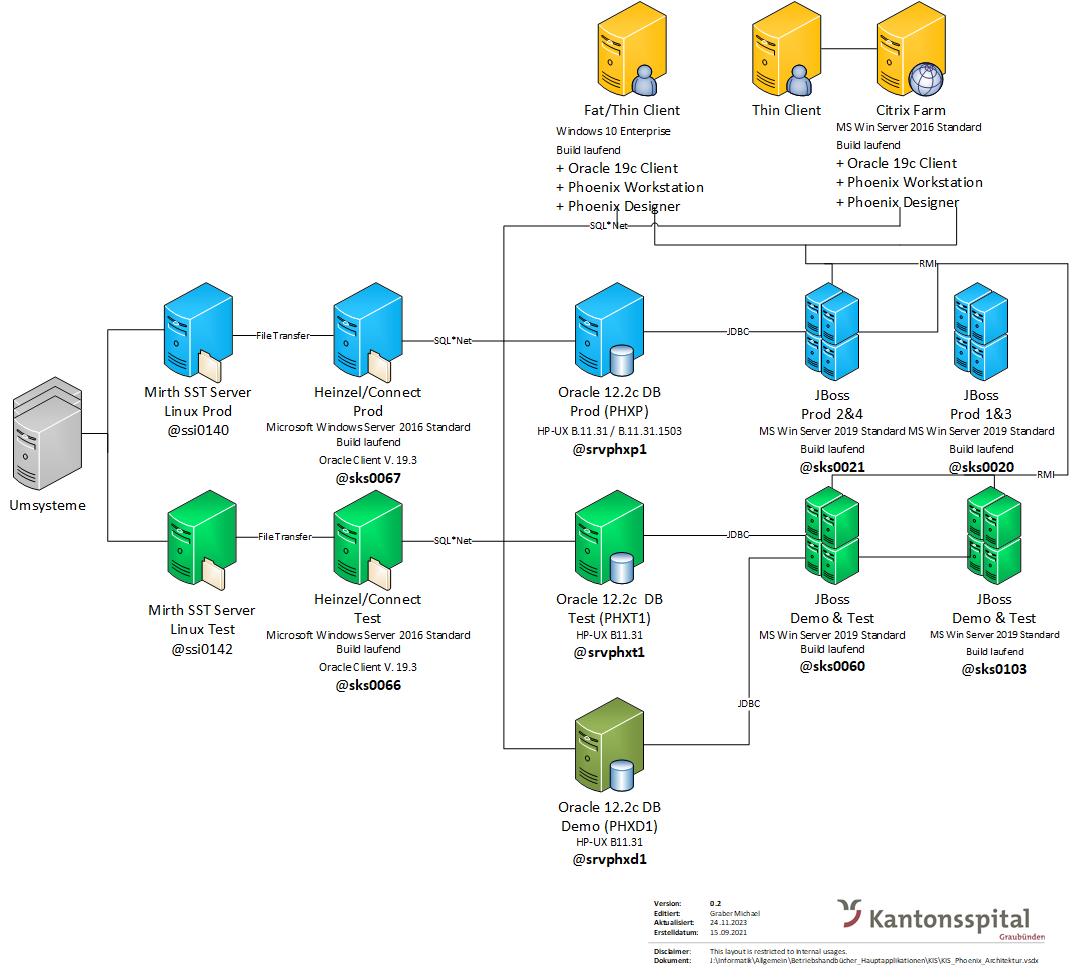
\includegraphics[width=1\linewidth]{source/introduction/KIS_Phoenix_Architektur}
        \caption{Architektur KIS Phoenix\cite{KFDFYH5H}}
        \label{fig:architektur-kis-phoenix}
    \end{figure}
\end{flushleft}
\begin{flushleft}
    Das Test1 und Demosystem hat je einen JBoss-Node auf einer Seite, das Test2 hat nur einen Node auf einem Server.
    Das Produktivsystem hat je Site zwei Nodes, also insgesamt vier Nodes.
\end{flushleft}
\begin{flushleft}
    Die Verzeichnisstruktur sieht dabei wie folgt aus:

%    \dirtree{%
%    .1 spam.
%    .2 ham.
%    .2 eggs.
%    .3 more spam.
%    .3 dead parrots.
%    }

%    \dirtree{%
%    .1 Laufwerk.
%    .2 {phoenix\_server\_system\_version}.
%    .3 node.
%    .4 standalone.
%    .5 log.
%    .6 server.log.
%    }

%    \dirtree{%
%
%    .1 spam.
%    .2 ham.
%    .2 eggs.
%    .3 more spam.
%    .3 dead parrots.
%%    .4 potatoes.
%    }

    \dirtree{%
        .1 /.
        .2 laufwerk.
        .3 phoenix-server-<system>-<version>.
        .4 <node>.
        .5 standalone.
        .6 log.
        .7 server.log.
    }

    \begin{mdframed}
    Meistens existieren pro Node die Verzeichnisse meherer Versionen, üblicherweise immer die der aktuellen und vorangehenden Version.\\Daher aufpassen in welchem Verzeichnis man ist!
    \end{mdframed}

    Auf jedem Server wurde zudem \textit{baretail.exe} installiert, ein Logging-Tool welches eine Echtzeitüberwachung der Logs ermöglicht.
    Leider ist es nicht auf jedem Server gleich installiert sondern individuell.

    Die genaue Konfiguration sieht wie folgt aus:
\end{flushleft}
    % Please add the following required packages to your document preamble:
    % \usepackage{booktabs}
    % \usepackage{graphicx}
    % \usepackage{lscape}
    \begin{landscape}
    \begin{table}[]
    \centering
    \resizebox{\columnwidth}{!}{%
    \begin{tabular}{@{}lccccccccccc@{}}
    \toprule
    \textbf{Typ}                                                     & \textbf{Applikationsserver} & \textbf{}                & \textbf{}                & \textbf{}                & \multicolumn{5}{c}{}                                                                                                                      & \multicolumn{2}{c}{\textbf{Schnittstellenserver}} \\ \midrule
    \textbf{\begin{tabular}[c]{@{}l@{}}Systeme\\ Rolle\end{tabular}} & \multicolumn{2}{c}{\textbf{Produktion}}                & \multicolumn{2}{c}{\textbf{Produktion}}             & \multicolumn{5}{c}{Test- und Demosystem Test- und Demosystem}                                                                             & \textbf{Produktion}        & \textbf{Test}        \\ \midrule
    \multicolumn{1}{l|}{\textbf{Physikalischer Hostname}}            & \multicolumn{2}{c}{sks0020}                            & \multicolumn{2}{c}{sks0021}                         & \multicolumn{3}{c}{sks0060}                                                       & \multicolumn{2}{c}{sks0103}                           & sks0067                    & sks0066              \\
    \multicolumn{1}{l|}{\textbf{IP Adresse phy. Host}}               & \multicolumn{2}{c}{10.0.22.43}                         & \multicolumn{2}{c}{10.0.22.44}                      & \multicolumn{3}{c}{10.0.22.52}                                                    &                           & 10.0.22.15                & 10.0.22.54                 & 10.0.22.53           \\
    \multicolumn{1}{l|}{\textbf{IP Submask}}                         & \multicolumn{11}{c}{255.255.255.0}                                                                                                                                                                                                                                                                           \\
    \multicolumn{1}{l|}{\textbf{Gateway}}                            & \multicolumn{11}{c}{10.0.22.1}                                                                                                                                                                                                                                                                               \\
    \multicolumn{1}{l|}{\textbf{DNS 1}}                              & \multicolumn{11}{c}{10.0.16.163}                                                                                                                                                                                                                                                                             \\
    \multicolumn{1}{l|}{\textbf{DNS 2}}                              & \multicolumn{11}{c}{10.0.16.163}                                                                                                                                                                                                                                                                             \\
    \multicolumn{1}{l|}{\textbf{Timeserver}}                         & \multicolumn{11}{c}{10.10.146.196}                                                                                                                                                                                                                                                                           \\
    \multicolumn{1}{l|}{\textbf{JBoss Nodes}}                        & prod1                       & prod3                    & prod2                    & prod4                    & demo11                    & test11                    & test21                    & demo12                    & test12                    &                            &                      \\
    \multicolumn{1}{l|}{\textbf{Windows Services}}                   & PhoenixJBossEAP\_prod\_1    & PhoenixJBossEAP\_prod\_3 & PhoenixJBossEAP\_prod\_2 & PhoenixJBossEAP\_prod\_4 & PhoenixJBossEAP\_demo1\_1 & PhoenixJBossEAP\_test1\_1 & PhoenixJBossEAP\_test2\_1 & PhoenixJBossEAP\_demo1\_2 & PhoenixJBossEAP\_test1\_2 &                            &                      \\ \bottomrule
    \end{tabular}%
    }
    \caption{Spezifikationen KIS Phoenix Applikations- und Schnittstellenserver}
    \label{tab:kis-phoenix-server-specs}
    \end{table}
    \end{landscape}
%\end{flushleft}
    %! Author = itgramic
%! Date = 11.10.23

% Preamble
%\begin{flushleft}
{
    \hypersetup{hidelinks}
    \listoffigures
}
%\end{flushleft}

\pagestyle{headings}
\thispagestyle{fancy}
%\begin{flushleft}
{
    \hypersetup{hidelinks}
    \listoftables
    \thispagestyle{fancy}
}
%\end{flushleft}
\pagestyle{headings}
\thispagestyle{fancy}

%\begin{flushleft}
{
    \cleardoublepage
    \renewcommand{\bibsetup}{\thispagestyle{fancy}}

    \printbibliography
}
%\end{flushleft}
%\begin{flushleft}
{
    \renewcommand*\glossarypreamble{\thispagestyle{fancy}}
    \printnoidxglossaries
}
%\end{flushleft}

\end{document}